%this file is the second report
%a % comment anything after % until the end of the line

%minimum references to begin our article
\documentclass[12pt]{article}
\usepackage[english]{babel}
\usepackage[utf8]{inputenc}
\usepackage[T1]{fontenc}
\usepackage{graphicx}
\usepackage{fancyhdr}
\usepackage{hyperref}
\usepackage{float}
\usepackage{enumitem}
\usepackage{amsmath}
\usepackage[margin=1in]{geometry}
\usepackage{indentfirst}
\usepackage{titlesec}
\usepackage{verbatim}
\usepackage{url}
\usepackage{rotating}
\usepackage{caption}

\usepackage{pdfpages}
\newcommand{\sectionbreak}{\clearpage}

%\setlength{\parskip}{10pt plus 1pt minus 1pt} %Adds spacing between paragraphs 
\usepackage{parskip}
\setlength{\parindent}{15pt}

\pagestyle{fancy}
%\cfoot{Fast and furious game playing: Monte Carlo drift}
% the last extension makes it possible to add images

%presentation of the document
\title{Fast and Furious Game Playing: Monte Carlo Drift\smallbreak Conception report} %not sure about the name of this report
\author{Prateek \textsc{Bhatnagar}, Gabriel \textsc{Prevosto}, \\
        Benoît \textsc{Viguier} \\
        \\
        Supervisors: Nikolaos \textsc{Parlavantzas}, Christian \textsc{Raymond}}
\date{02/02/2015}
\setlength\parindent{15pt}
\begin{document}
\maketitle

\begin{figure}[!h] 
\centerline{\includegraphics[scale=0.50]{Pictures/arimaa}}
\end{figure}
\newpage

%to add a table of contents
\tableofcontents
\newpage


\section{Introduction}				\label{sec:introduction} 		The base algorithm is a simple implementation of the MCTS algorithm. All the functions related to it are included in the mcts namespace.
It take as a parameter the abstract class \textit{TheGame}, the position (\textit{Bitboard}) to start the search with and an object (\textit{MctsArg}) to set the parameter to the MCTS algorithm such as the time to search on, the depth of the tree, the number of simulation to run and the number of nodes to create in the tree.
The following Class Diagram represent the links between the differents kinds of objects.
\begin{figure}[H] 
\centerline{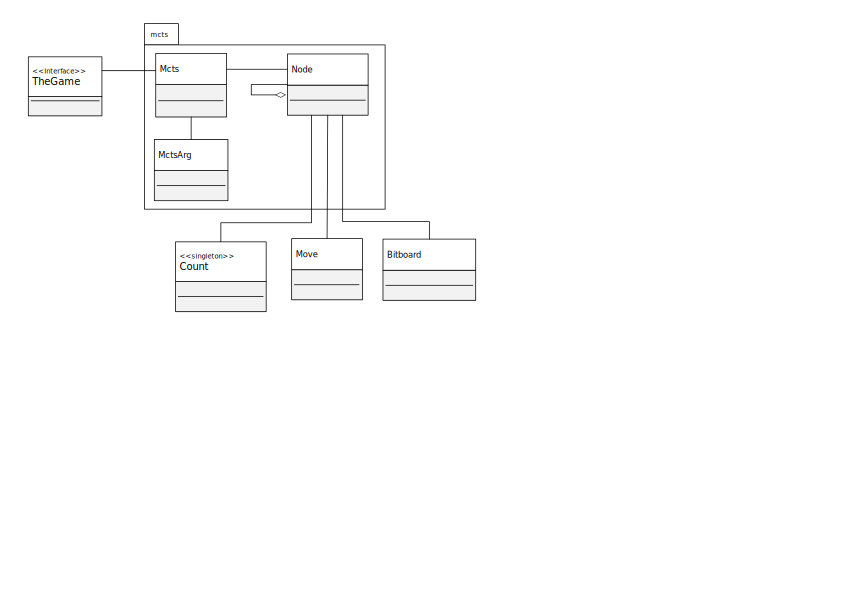
\includegraphics[scale=1]{Base_Algorithm/Img/MCTSsimple.png}}
\caption{\label{fig:MCTSClassDiagram}\textit{Class Diagram of the mcts package}}
\end{figure}
The Object Node represent the tree, it is stored as an array in the mcts object. A detailed implementation is provided in the Data Structure part.\\
The singleton \textit{Count} is used for the statistics (such as the number of leaves, nodes created and the number of simultions run). Whilst providing statistics it also make sure that no  memory leaks are happening, monitoring the creation and destructions of the main objects.\\ 
The following figure represent the order of the call for the main function while providing some details about the implementation.
\begin{figure}[H]
\centerline{\includegraphics[scale=0.70]{Base_Algorithm/Img/Algorithm.png}}
\caption{\label{fig:MCTSAlgorithm}\textit{Monte Carlo algorithm}}
\end{figure}
\noindent
\textit{\textbf{explore}} : start the tree exploration.
\medskip\\
\textit{\textbf{UpdateNode}} : make the the node has children and update its terminal value if required.
\medskip\\
\textit{\textbf{select\_child\_UCT}} : go through all the children of a node and return the one with the highest result at the UCT function (refer to the \textit{pre-analysis report, part 3.4.4}).
\medskip\\
\textit{\textbf{playRandom}} : start to run the random simulations and return the winner/tie.
\medskip\\
\textit{\textbf{update}} : update the node statistics and feedback the result to its parents.
\medskip\\
\textit{\textbf{forceSetUCT}} : In the event of a winning move, the uct value is set to 10 in order to make sure that each and every further explorations go through that node.
\medskip\\
\textit{\textbf{feedbackWinningMove}} : feedback the winning move to its parent, we don't want to go to that position because it would be a winning strategy for the opponent.
\medskip\\
\textit{\textbf{updateLosingParent}} : in the event of all the children of the parent being a losing move, update it's UCT value to winning strategy to propagate the results.
\medskip\\
\textit{\textbf{select\_child\_WR}} : return the child with the highest win rate.\\


\newpage
\section{Base algorithm}			\label{sec:Algo}			The base algorithm is a simple implementation of the MCTS algorithm. All the functions related to it are included in the mcts namespace.
It take as a parameter the abstract class \textit{TheGame}, the position (\textit{Bitboard}) to start the search with and an object (\textit{MctsArg}) to set the parameter to the MCTS algorithm such as the time to search on, the depth of the tree, the number of simulation to run and the number of nodes to create in the tree.
The following Class Diagram represent the links between the differents kinds of objects.
\begin{figure}[H] 
\centerline{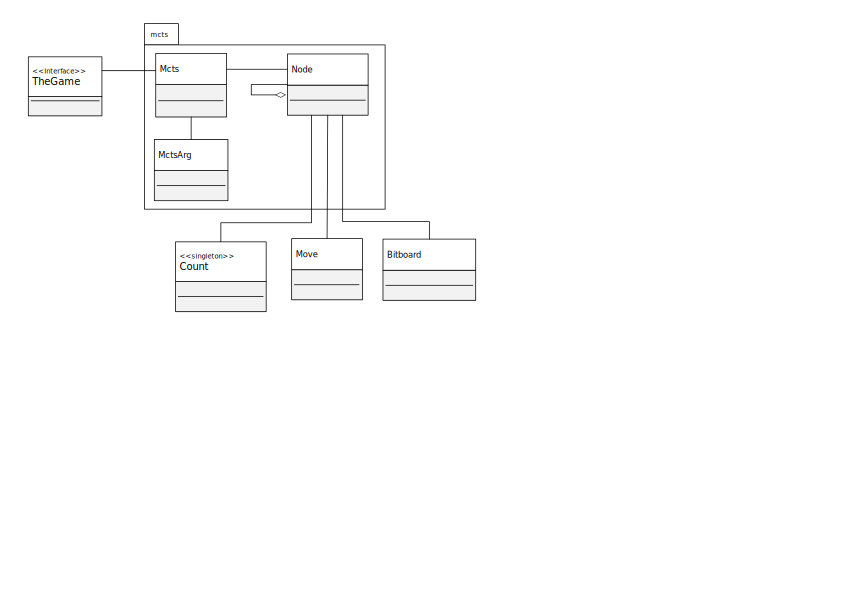
\includegraphics[scale=1]{Base_Algorithm/Img/MCTSsimple.png}}
\caption{\label{fig:MCTSClassDiagram}\textit{Class Diagram of the mcts package}}
\end{figure}
The Object Node represent the tree, it is stored as an array in the mcts object. A detailed implementation is provided in the Data Structure part.\\
The singleton \textit{Count} is used for the statistics (such as the number of leaves, nodes created and the number of simultions run). Whilst providing statistics it also make sure that no  memory leaks are happening, monitoring the creation and destructions of the main objects.\\ 
The following figure represent the order of the call for the main function while providing some details about the implementation.
\begin{figure}[H]
\centerline{\includegraphics[scale=0.70]{Base_Algorithm/Img/Algorithm.png}}
\caption{\label{fig:MCTSAlgorithm}\textit{Monte Carlo algorithm}}
\end{figure}
\noindent
\textit{\textbf{explore}} : start the tree exploration.
\medskip\\
\textit{\textbf{UpdateNode}} : make the the node has children and update its terminal value if required.
\medskip\\
\textit{\textbf{select\_child\_UCT}} : go through all the children of a node and return the one with the highest result at the UCT function (refer to the \textit{pre-analysis report, part 3.4.4}).
\medskip\\
\textit{\textbf{playRandom}} : start to run the random simulations and return the winner/tie.
\medskip\\
\textit{\textbf{update}} : update the node statistics and feedback the result to its parents.
\medskip\\
\textit{\textbf{forceSetUCT}} : In the event of a winning move, the uct value is set to 10 in order to make sure that each and every further explorations go through that node.
\medskip\\
\textit{\textbf{feedbackWinningMove}} : feedback the winning move to its parent, we don't want to go to that position because it would be a winning strategy for the opponent.
\medskip\\
\textit{\textbf{updateLosingParent}} : in the event of all the children of the parent being a losing move, update it's UCT value to winning strategy to propagate the results.
\medskip\\
\textit{\textbf{select\_child\_WR}} : return the child with the highest win rate.\\


\newpage
\section{Data structure}			\label{sec:data}			The base algorithm is a simple implementation of the MCTS algorithm. All the functions related to it are included in the mcts namespace.
It take as a parameter the abstract class \textit{TheGame}, the position (\textit{Bitboard}) to start the search with and an object (\textit{MctsArg}) to set the parameter to the MCTS algorithm such as the time to search on, the depth of the tree, the number of simulation to run and the number of nodes to create in the tree.
The following Class Diagram represent the links between the differents kinds of objects.
\begin{figure}[H] 
\centerline{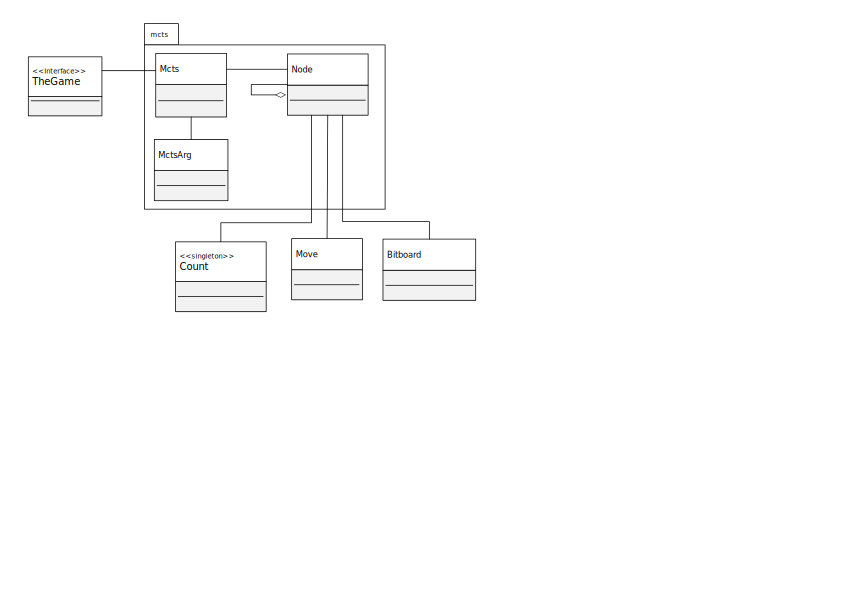
\includegraphics[scale=1]{Base_Algorithm/Img/MCTSsimple.png}}
\caption{\label{fig:MCTSClassDiagram}\textit{Class Diagram of the mcts package}}
\end{figure}
The Object Node represent the tree, it is stored as an array in the mcts object. A detailed implementation is provided in the Data Structure part.\\
The singleton \textit{Count} is used for the statistics (such as the number of leaves, nodes created and the number of simultions run). Whilst providing statistics it also make sure that no  memory leaks are happening, monitoring the creation and destructions of the main objects.\\ 
The following figure represent the order of the call for the main function while providing some details about the implementation.
\begin{figure}[H]
\centerline{\includegraphics[scale=0.70]{Base_Algorithm/Img/Algorithm.png}}
\caption{\label{fig:MCTSAlgorithm}\textit{Monte Carlo algorithm}}
\end{figure}
\noindent
\textit{\textbf{explore}} : start the tree exploration.
\medskip\\
\textit{\textbf{UpdateNode}} : make the the node has children and update its terminal value if required.
\medskip\\
\textit{\textbf{select\_child\_UCT}} : go through all the children of a node and return the one with the highest result at the UCT function (refer to the \textit{pre-analysis report, part 3.4.4}).
\medskip\\
\textit{\textbf{playRandom}} : start to run the random simulations and return the winner/tie.
\medskip\\
\textit{\textbf{update}} : update the node statistics and feedback the result to its parents.
\medskip\\
\textit{\textbf{forceSetUCT}} : In the event of a winning move, the uct value is set to 10 in order to make sure that each and every further explorations go through that node.
\medskip\\
\textit{\textbf{feedbackWinningMove}} : feedback the winning move to its parent, we don't want to go to that position because it would be a winning strategy for the opponent.
\medskip\\
\textit{\textbf{updateLosingParent}} : in the event of all the children of the parent being a losing move, update it's UCT value to winning strategy to propagate the results.
\medskip\\
\textit{\textbf{select\_child\_WR}} : return the child with the highest win rate.\\


\newpage
\section{Parallelisation strategy}		\label{sec:paralstrat}			The base algorithm is a simple implementation of the MCTS algorithm. All the functions related to it are included in the mcts namespace.
It take as a parameter the abstract class \textit{TheGame}, the position (\textit{Bitboard}) to start the search with and an object (\textit{MctsArg}) to set the parameter to the MCTS algorithm such as the time to search on, the depth of the tree, the number of simulation to run and the number of nodes to create in the tree.
The following Class Diagram represent the links between the differents kinds of objects.
\begin{figure}[H] 
\centerline{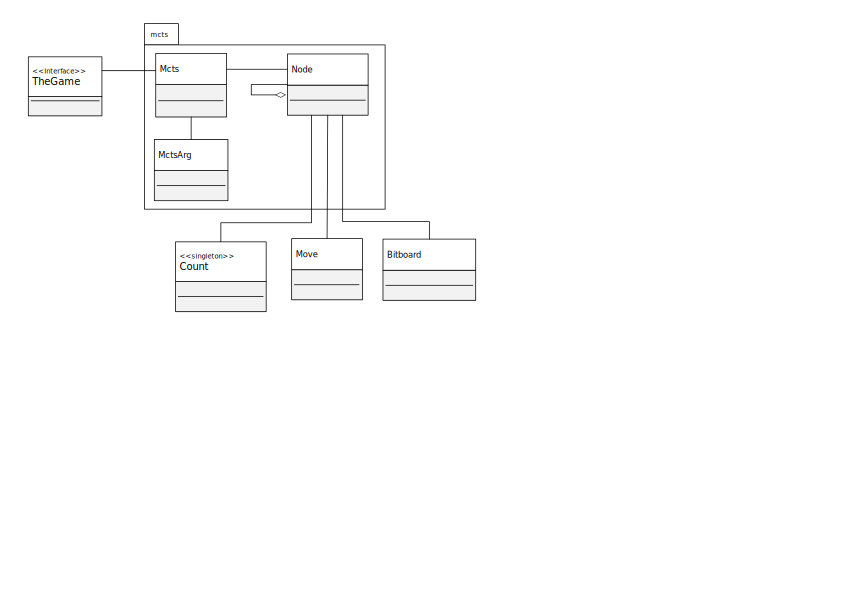
\includegraphics[scale=1]{Base_Algorithm/Img/MCTSsimple.png}}
\caption{\label{fig:MCTSClassDiagram}\textit{Class Diagram of the mcts package}}
\end{figure}
The Object Node represent the tree, it is stored as an array in the mcts object. A detailed implementation is provided in the Data Structure part.\\
The singleton \textit{Count} is used for the statistics (such as the number of leaves, nodes created and the number of simultions run). Whilst providing statistics it also make sure that no  memory leaks are happening, monitoring the creation and destructions of the main objects.\\ 
The following figure represent the order of the call for the main function while providing some details about the implementation.
\begin{figure}[H]
\centerline{\includegraphics[scale=0.70]{Base_Algorithm/Img/Algorithm.png}}
\caption{\label{fig:MCTSAlgorithm}\textit{Monte Carlo algorithm}}
\end{figure}
\noindent
\textit{\textbf{explore}} : start the tree exploration.
\medskip\\
\textit{\textbf{UpdateNode}} : make the the node has children and update its terminal value if required.
\medskip\\
\textit{\textbf{select\_child\_UCT}} : go through all the children of a node and return the one with the highest result at the UCT function (refer to the \textit{pre-analysis report, part 3.4.4}).
\medskip\\
\textit{\textbf{playRandom}} : start to run the random simulations and return the winner/tie.
\medskip\\
\textit{\textbf{update}} : update the node statistics and feedback the result to its parents.
\medskip\\
\textit{\textbf{forceSetUCT}} : In the event of a winning move, the uct value is set to 10 in order to make sure that each and every further explorations go through that node.
\medskip\\
\textit{\textbf{feedbackWinningMove}} : feedback the winning move to its parent, we don't want to go to that position because it would be a winning strategy for the opponent.
\medskip\\
\textit{\textbf{updateLosingParent}} : in the event of all the children of the parent being a losing move, update it's UCT value to winning strategy to propagate the results.
\medskip\\
\textit{\textbf{select\_child\_WR}} : return the child with the highest win rate.\\


\newpage
\section{Parallelisation frameworks}		\label{sec:paralframew}
	\subsection{OpenMP}			\label{sec:openmp}			The base algorithm is a simple implementation of the MCTS algorithm. All the functions related to it are included in the mcts namespace.
It take as a parameter the abstract class \textit{TheGame}, the position (\textit{Bitboard}) to start the search with and an object (\textit{MctsArg}) to set the parameter to the MCTS algorithm such as the time to search on, the depth of the tree, the number of simulation to run and the number of nodes to create in the tree.
The following Class Diagram represent the links between the differents kinds of objects.
\begin{figure}[H] 
\centerline{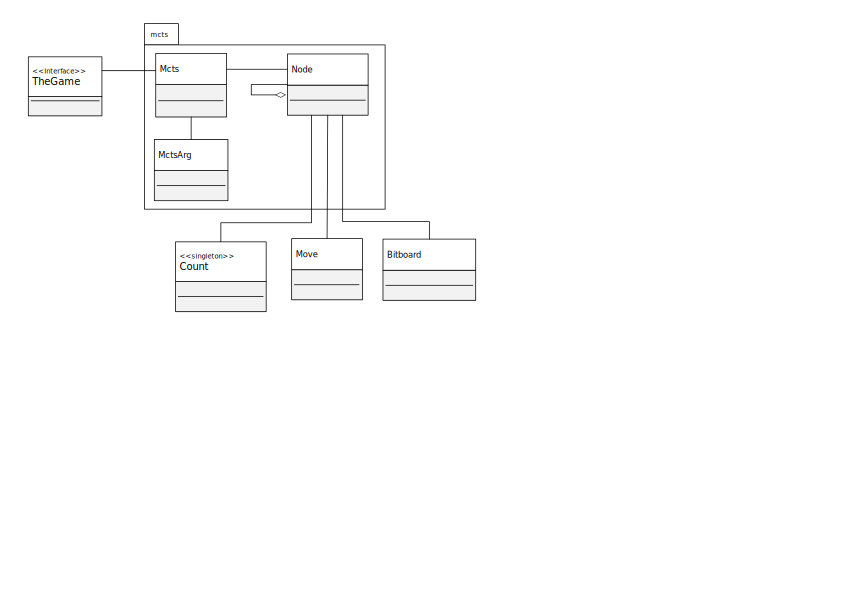
\includegraphics[scale=1]{Base_Algorithm/Img/MCTSsimple.png}}
\caption{\label{fig:MCTSClassDiagram}\textit{Class Diagram of the mcts package}}
\end{figure}
The Object Node represent the tree, it is stored as an array in the mcts object. A detailed implementation is provided in the Data Structure part.\\
The singleton \textit{Count} is used for the statistics (such as the number of leaves, nodes created and the number of simultions run). Whilst providing statistics it also make sure that no  memory leaks are happening, monitoring the creation and destructions of the main objects.\\ 
The following figure represent the order of the call for the main function while providing some details about the implementation.
\begin{figure}[H]
\centerline{\includegraphics[scale=0.70]{Base_Algorithm/Img/Algorithm.png}}
\caption{\label{fig:MCTSAlgorithm}\textit{Monte Carlo algorithm}}
\end{figure}
\noindent
\textit{\textbf{explore}} : start the tree exploration.
\medskip\\
\textit{\textbf{UpdateNode}} : make the the node has children and update its terminal value if required.
\medskip\\
\textit{\textbf{select\_child\_UCT}} : go through all the children of a node and return the one with the highest result at the UCT function (refer to the \textit{pre-analysis report, part 3.4.4}).
\medskip\\
\textit{\textbf{playRandom}} : start to run the random simulations and return the winner/tie.
\medskip\\
\textit{\textbf{update}} : update the node statistics and feedback the result to its parents.
\medskip\\
\textit{\textbf{forceSetUCT}} : In the event of a winning move, the uct value is set to 10 in order to make sure that each and every further explorations go through that node.
\medskip\\
\textit{\textbf{feedbackWinningMove}} : feedback the winning move to its parent, we don't want to go to that position because it would be a winning strategy for the opponent.
\medskip\\
\textit{\textbf{updateLosingParent}} : in the event of all the children of the parent being a losing move, update it's UCT value to winning strategy to propagate the results.
\medskip\\
\textit{\textbf{select\_child\_WR}} : return the child with the highest win rate.\\

	\subsection{MPI}			\label{sec:mpi}				The base algorithm is a simple implementation of the MCTS algorithm. All the functions related to it are included in the mcts namespace.
It take as a parameter the abstract class \textit{TheGame}, the position (\textit{Bitboard}) to start the search with and an object (\textit{MctsArg}) to set the parameter to the MCTS algorithm such as the time to search on, the depth of the tree, the number of simulation to run and the number of nodes to create in the tree.
The following Class Diagram represent the links between the differents kinds of objects.
\begin{figure}[H] 
\centerline{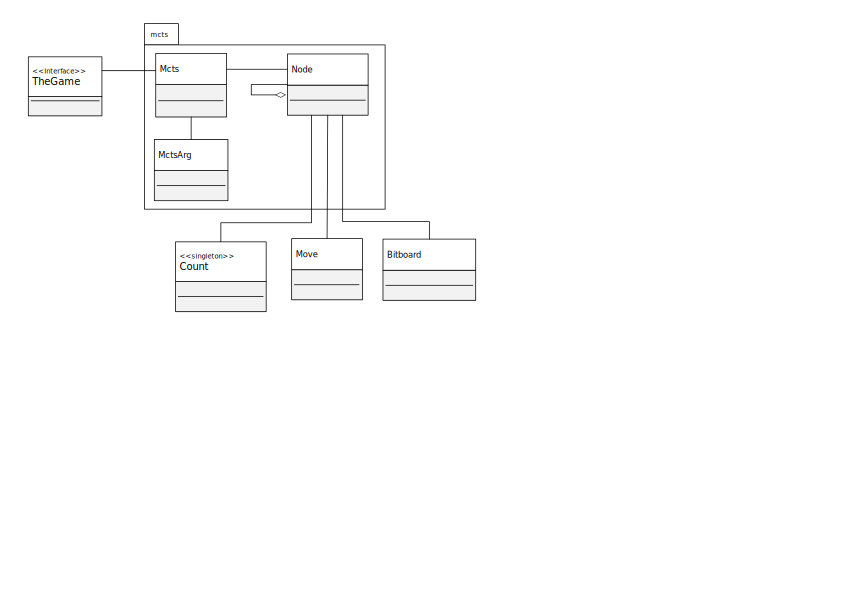
\includegraphics[scale=1]{Base_Algorithm/Img/MCTSsimple.png}}
\caption{\label{fig:MCTSClassDiagram}\textit{Class Diagram of the mcts package}}
\end{figure}
The Object Node represent the tree, it is stored as an array in the mcts object. A detailed implementation is provided in the Data Structure part.\\
The singleton \textit{Count} is used for the statistics (such as the number of leaves, nodes created and the number of simultions run). Whilst providing statistics it also make sure that no  memory leaks are happening, monitoring the creation and destructions of the main objects.\\ 
The following figure represent the order of the call for the main function while providing some details about the implementation.
\begin{figure}[H]
\centerline{\includegraphics[scale=0.70]{Base_Algorithm/Img/Algorithm.png}}
\caption{\label{fig:MCTSAlgorithm}\textit{Monte Carlo algorithm}}
\end{figure}
\noindent
\textit{\textbf{explore}} : start the tree exploration.
\medskip\\
\textit{\textbf{UpdateNode}} : make the the node has children and update its terminal value if required.
\medskip\\
\textit{\textbf{select\_child\_UCT}} : go through all the children of a node and return the one with the highest result at the UCT function (refer to the \textit{pre-analysis report, part 3.4.4}).
\medskip\\
\textit{\textbf{playRandom}} : start to run the random simulations and return the winner/tie.
\medskip\\
\textit{\textbf{update}} : update the node statistics and feedback the result to its parents.
\medskip\\
\textit{\textbf{forceSetUCT}} : In the event of a winning move, the uct value is set to 10 in order to make sure that each and every further explorations go through that node.
\medskip\\
\textit{\textbf{feedbackWinningMove}} : feedback the winning move to its parent, we don't want to go to that position because it would be a winning strategy for the opponent.
\medskip\\
\textit{\textbf{updateLosingParent}} : in the event of all the children of the parent being a losing move, update it's UCT value to winning strategy to propagate the results.
\medskip\\
\textit{\textbf{select\_child\_WR}} : return the child with the highest win rate.\\

	\subsection{CAF}			\label{sec:caf}				The base algorithm is a simple implementation of the MCTS algorithm. All the functions related to it are included in the mcts namespace.
It take as a parameter the abstract class \textit{TheGame}, the position (\textit{Bitboard}) to start the search with and an object (\textit{MctsArg}) to set the parameter to the MCTS algorithm such as the time to search on, the depth of the tree, the number of simulation to run and the number of nodes to create in the tree.
The following Class Diagram represent the links between the differents kinds of objects.
\begin{figure}[H] 
\centerline{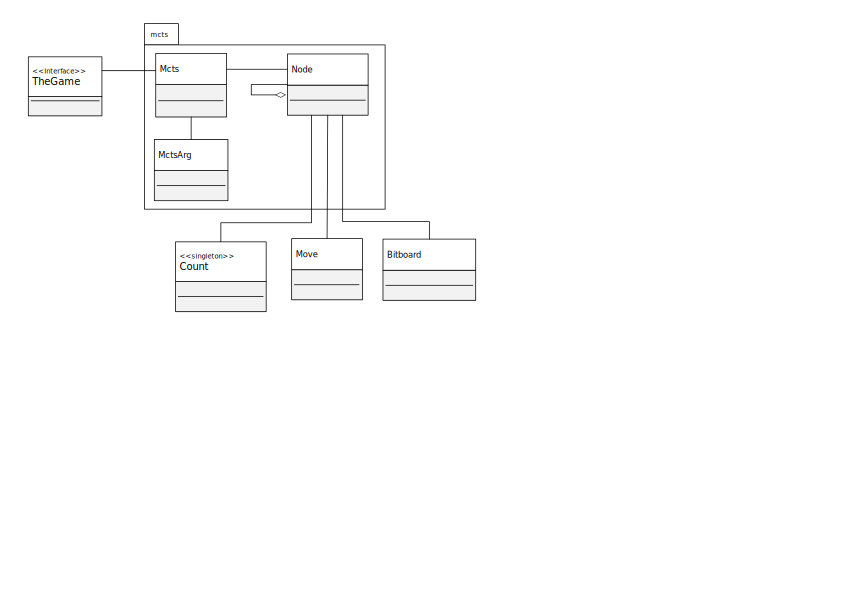
\includegraphics[scale=1]{Base_Algorithm/Img/MCTSsimple.png}}
\caption{\label{fig:MCTSClassDiagram}\textit{Class Diagram of the mcts package}}
\end{figure}
The Object Node represent the tree, it is stored as an array in the mcts object. A detailed implementation is provided in the Data Structure part.\\
The singleton \textit{Count} is used for the statistics (such as the number of leaves, nodes created and the number of simultions run). Whilst providing statistics it also make sure that no  memory leaks are happening, monitoring the creation and destructions of the main objects.\\ 
The following figure represent the order of the call for the main function while providing some details about the implementation.
\begin{figure}[H]
\centerline{\includegraphics[scale=0.70]{Base_Algorithm/Img/Algorithm.png}}
\caption{\label{fig:MCTSAlgorithm}\textit{Monte Carlo algorithm}}
\end{figure}
\noindent
\textit{\textbf{explore}} : start the tree exploration.
\medskip\\
\textit{\textbf{UpdateNode}} : make the the node has children and update its terminal value if required.
\medskip\\
\textit{\textbf{select\_child\_UCT}} : go through all the children of a node and return the one with the highest result at the UCT function (refer to the \textit{pre-analysis report, part 3.4.4}).
\medskip\\
\textit{\textbf{playRandom}} : start to run the random simulations and return the winner/tie.
\medskip\\
\textit{\textbf{update}} : update the node statistics and feedback the result to its parents.
\medskip\\
\textit{\textbf{forceSetUCT}} : In the event of a winning move, the uct value is set to 10 in order to make sure that each and every further explorations go through that node.
\medskip\\
\textit{\textbf{feedbackWinningMove}} : feedback the winning move to its parent, we don't want to go to that position because it would be a winning strategy for the opponent.
\medskip\\
\textit{\textbf{updateLosingParent}} : in the event of all the children of the parent being a losing move, update it's UCT value to winning strategy to propagate the results.
\medskip\\
\textit{\textbf{select\_child\_WR}} : return the child with the highest win rate.\\


\newpage
\section{Graphical User Interface}		\label{sec:gui}				The base algorithm is a simple implementation of the MCTS algorithm. All the functions related to it are included in the mcts namespace.
It take as a parameter the abstract class \textit{TheGame}, the position (\textit{Bitboard}) to start the search with and an object (\textit{MctsArg}) to set the parameter to the MCTS algorithm such as the time to search on, the depth of the tree, the number of simulation to run and the number of nodes to create in the tree.
The following Class Diagram represent the links between the differents kinds of objects.
\begin{figure}[H] 
\centerline{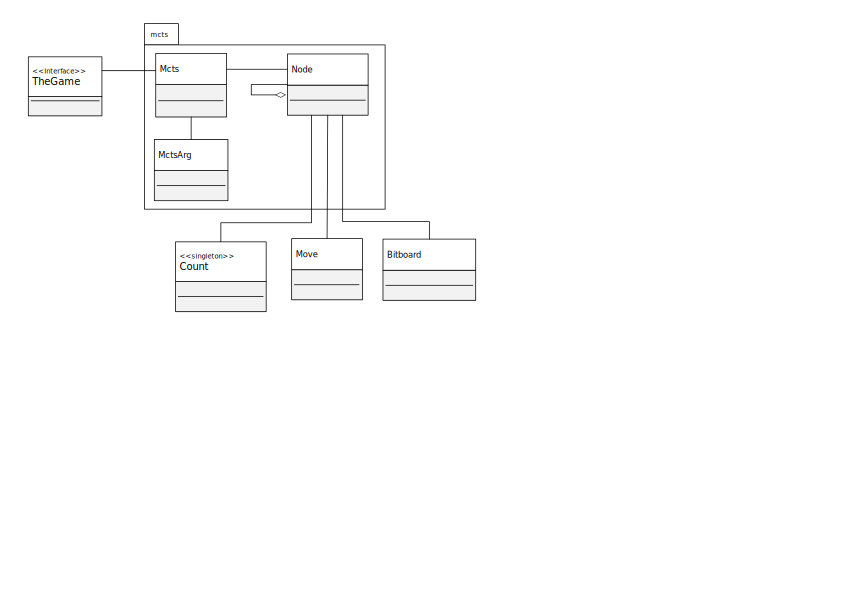
\includegraphics[scale=1]{Base_Algorithm/Img/MCTSsimple.png}}
\caption{\label{fig:MCTSClassDiagram}\textit{Class Diagram of the mcts package}}
\end{figure}
The Object Node represent the tree, it is stored as an array in the mcts object. A detailed implementation is provided in the Data Structure part.\\
The singleton \textit{Count} is used for the statistics (such as the number of leaves, nodes created and the number of simultions run). Whilst providing statistics it also make sure that no  memory leaks are happening, monitoring the creation and destructions of the main objects.\\ 
The following figure represent the order of the call for the main function while providing some details about the implementation.
\begin{figure}[H]
\centerline{\includegraphics[scale=0.70]{Base_Algorithm/Img/Algorithm.png}}
\caption{\label{fig:MCTSAlgorithm}\textit{Monte Carlo algorithm}}
\end{figure}
\noindent
\textit{\textbf{explore}} : start the tree exploration.
\medskip\\
\textit{\textbf{UpdateNode}} : make the the node has children and update its terminal value if required.
\medskip\\
\textit{\textbf{select\_child\_UCT}} : go through all the children of a node and return the one with the highest result at the UCT function (refer to the \textit{pre-analysis report, part 3.4.4}).
\medskip\\
\textit{\textbf{playRandom}} : start to run the random simulations and return the winner/tie.
\medskip\\
\textit{\textbf{update}} : update the node statistics and feedback the result to its parents.
\medskip\\
\textit{\textbf{forceSetUCT}} : In the event of a winning move, the uct value is set to 10 in order to make sure that each and every further explorations go through that node.
\medskip\\
\textit{\textbf{feedbackWinningMove}} : feedback the winning move to its parent, we don't want to go to that position because it would be a winning strategy for the opponent.
\medskip\\
\textit{\textbf{updateLosingParent}} : in the event of all the children of the parent being a losing move, update it's UCT value to winning strategy to propagate the results.
\medskip\\
\textit{\textbf{select\_child\_WR}} : return the child with the highest win rate.\\


\newpage
	\section{Conclusion}			\label{sec:conclusion}			The base algorithm is a simple implementation of the MCTS algorithm. All the functions related to it are included in the mcts namespace.
It take as a parameter the abstract class \textit{TheGame}, the position (\textit{Bitboard}) to start the search with and an object (\textit{MctsArg}) to set the parameter to the MCTS algorithm such as the time to search on, the depth of the tree, the number of simulation to run and the number of nodes to create in the tree.
The following Class Diagram represent the links between the differents kinds of objects.
\begin{figure}[H] 
\centerline{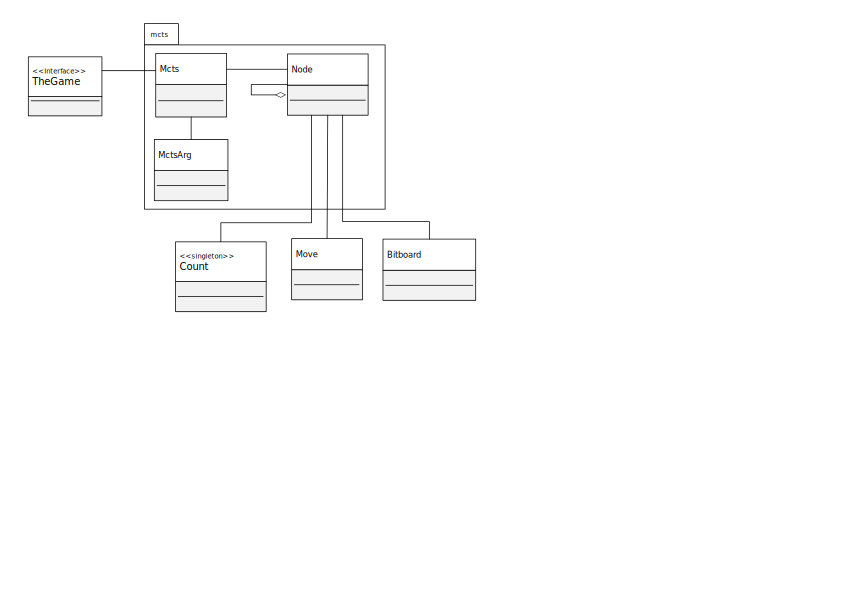
\includegraphics[scale=1]{Base_Algorithm/Img/MCTSsimple.png}}
\caption{\label{fig:MCTSClassDiagram}\textit{Class Diagram of the mcts package}}
\end{figure}
The Object Node represent the tree, it is stored as an array in the mcts object. A detailed implementation is provided in the Data Structure part.\\
The singleton \textit{Count} is used for the statistics (such as the number of leaves, nodes created and the number of simultions run). Whilst providing statistics it also make sure that no  memory leaks are happening, monitoring the creation and destructions of the main objects.\\ 
The following figure represent the order of the call for the main function while providing some details about the implementation.
\begin{figure}[H]
\centerline{\includegraphics[scale=0.70]{Base_Algorithm/Img/Algorithm.png}}
\caption{\label{fig:MCTSAlgorithm}\textit{Monte Carlo algorithm}}
\end{figure}
\noindent
\textit{\textbf{explore}} : start the tree exploration.
\medskip\\
\textit{\textbf{UpdateNode}} : make the the node has children and update its terminal value if required.
\medskip\\
\textit{\textbf{select\_child\_UCT}} : go through all the children of a node and return the one with the highest result at the UCT function (refer to the \textit{pre-analysis report, part 3.4.4}).
\medskip\\
\textit{\textbf{playRandom}} : start to run the random simulations and return the winner/tie.
\medskip\\
\textit{\textbf{update}} : update the node statistics and feedback the result to its parents.
\medskip\\
\textit{\textbf{forceSetUCT}} : In the event of a winning move, the uct value is set to 10 in order to make sure that each and every further explorations go through that node.
\medskip\\
\textit{\textbf{feedbackWinningMove}} : feedback the winning move to its parent, we don't want to go to that position because it would be a winning strategy for the opponent.
\medskip\\
\textit{\textbf{updateLosingParent}} : in the event of all the children of the parent being a losing move, update it's UCT value to winning strategy to propagate the results.
\medskip\\
\textit{\textbf{select\_child\_WR}} : return the child with the highest win rate.\\

\newpage


\newpage
	\section{Annexes}			\label{sec:annexes}			The base algorithm is a simple implementation of the MCTS algorithm. All the functions related to it are included in the mcts namespace.
It take as a parameter the abstract class \textit{TheGame}, the position (\textit{Bitboard}) to start the search with and an object (\textit{MctsArg}) to set the parameter to the MCTS algorithm such as the time to search on, the depth of the tree, the number of simulation to run and the number of nodes to create in the tree.
The following Class Diagram represent the links between the differents kinds of objects.
\begin{figure}[H] 
\centerline{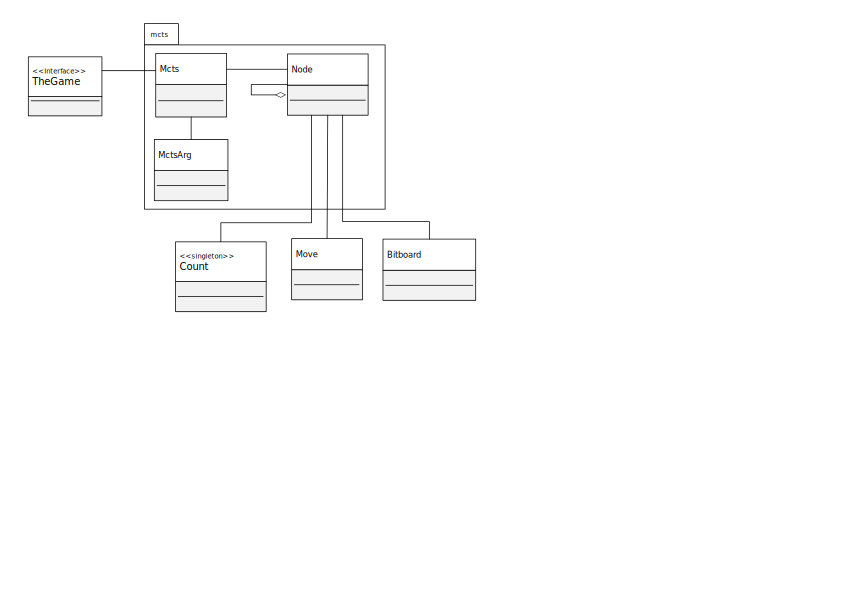
\includegraphics[scale=1]{Base_Algorithm/Img/MCTSsimple.png}}
\caption{\label{fig:MCTSClassDiagram}\textit{Class Diagram of the mcts package}}
\end{figure}
The Object Node represent the tree, it is stored as an array in the mcts object. A detailed implementation is provided in the Data Structure part.\\
The singleton \textit{Count} is used for the statistics (such as the number of leaves, nodes created and the number of simultions run). Whilst providing statistics it also make sure that no  memory leaks are happening, monitoring the creation and destructions of the main objects.\\ 
The following figure represent the order of the call for the main function while providing some details about the implementation.
\begin{figure}[H]
\centerline{\includegraphics[scale=0.70]{Base_Algorithm/Img/Algorithm.png}}
\caption{\label{fig:MCTSAlgorithm}\textit{Monte Carlo algorithm}}
\end{figure}
\noindent
\textit{\textbf{explore}} : start the tree exploration.
\medskip\\
\textit{\textbf{UpdateNode}} : make the the node has children and update its terminal value if required.
\medskip\\
\textit{\textbf{select\_child\_UCT}} : go through all the children of a node and return the one with the highest result at the UCT function (refer to the \textit{pre-analysis report, part 3.4.4}).
\medskip\\
\textit{\textbf{playRandom}} : start to run the random simulations and return the winner/tie.
\medskip\\
\textit{\textbf{update}} : update the node statistics and feedback the result to its parents.
\medskip\\
\textit{\textbf{forceSetUCT}} : In the event of a winning move, the uct value is set to 10 in order to make sure that each and every further explorations go through that node.
\medskip\\
\textit{\textbf{feedbackWinningMove}} : feedback the winning move to its parent, we don't want to go to that position because it would be a winning strategy for the opponent.
\medskip\\
\textit{\textbf{updateLosingParent}} : in the event of all the children of the parent being a losing move, update it's UCT value to winning strategy to propagate the results.
\medskip\\
\textit{\textbf{select\_child\_WR}} : return the child with the highest win rate.\\

\newpage

\bibliography{bibliography}
\bibliographystyle{plain}

\end{document}
